\section{Processing Guarantees}

	\noindent\textbf{Definition:} we have three modes of guarantees 
	\begin{itemize}
		\item at most once (weakest) : guaranteeing each message is processed at most once with a chance of getting lost
		\item at least once: guaranteeing processing each message at least once, with a chance of reprocessing some of the messages
		\item exactly once (strongest): guaranteeing each message being processed exactly one (no loss or reprocessing)
	\end{itemize}	 

	\noindent \textbf{Purpose:} This BB adds guarantees to the processing. Also, provides a mean to trade-off between performance and precise computing. As shown in \ref{fig:guarantees}, "at-most-once provides higher performance with lower latency and higher throughput, with more overhead being added as moving to "exactly-once". However, this comes at a cost of less precise processing with the possibility of loosing messages or processing the same message multiple times.
	
	\begin{figure}[h]
		\centering
		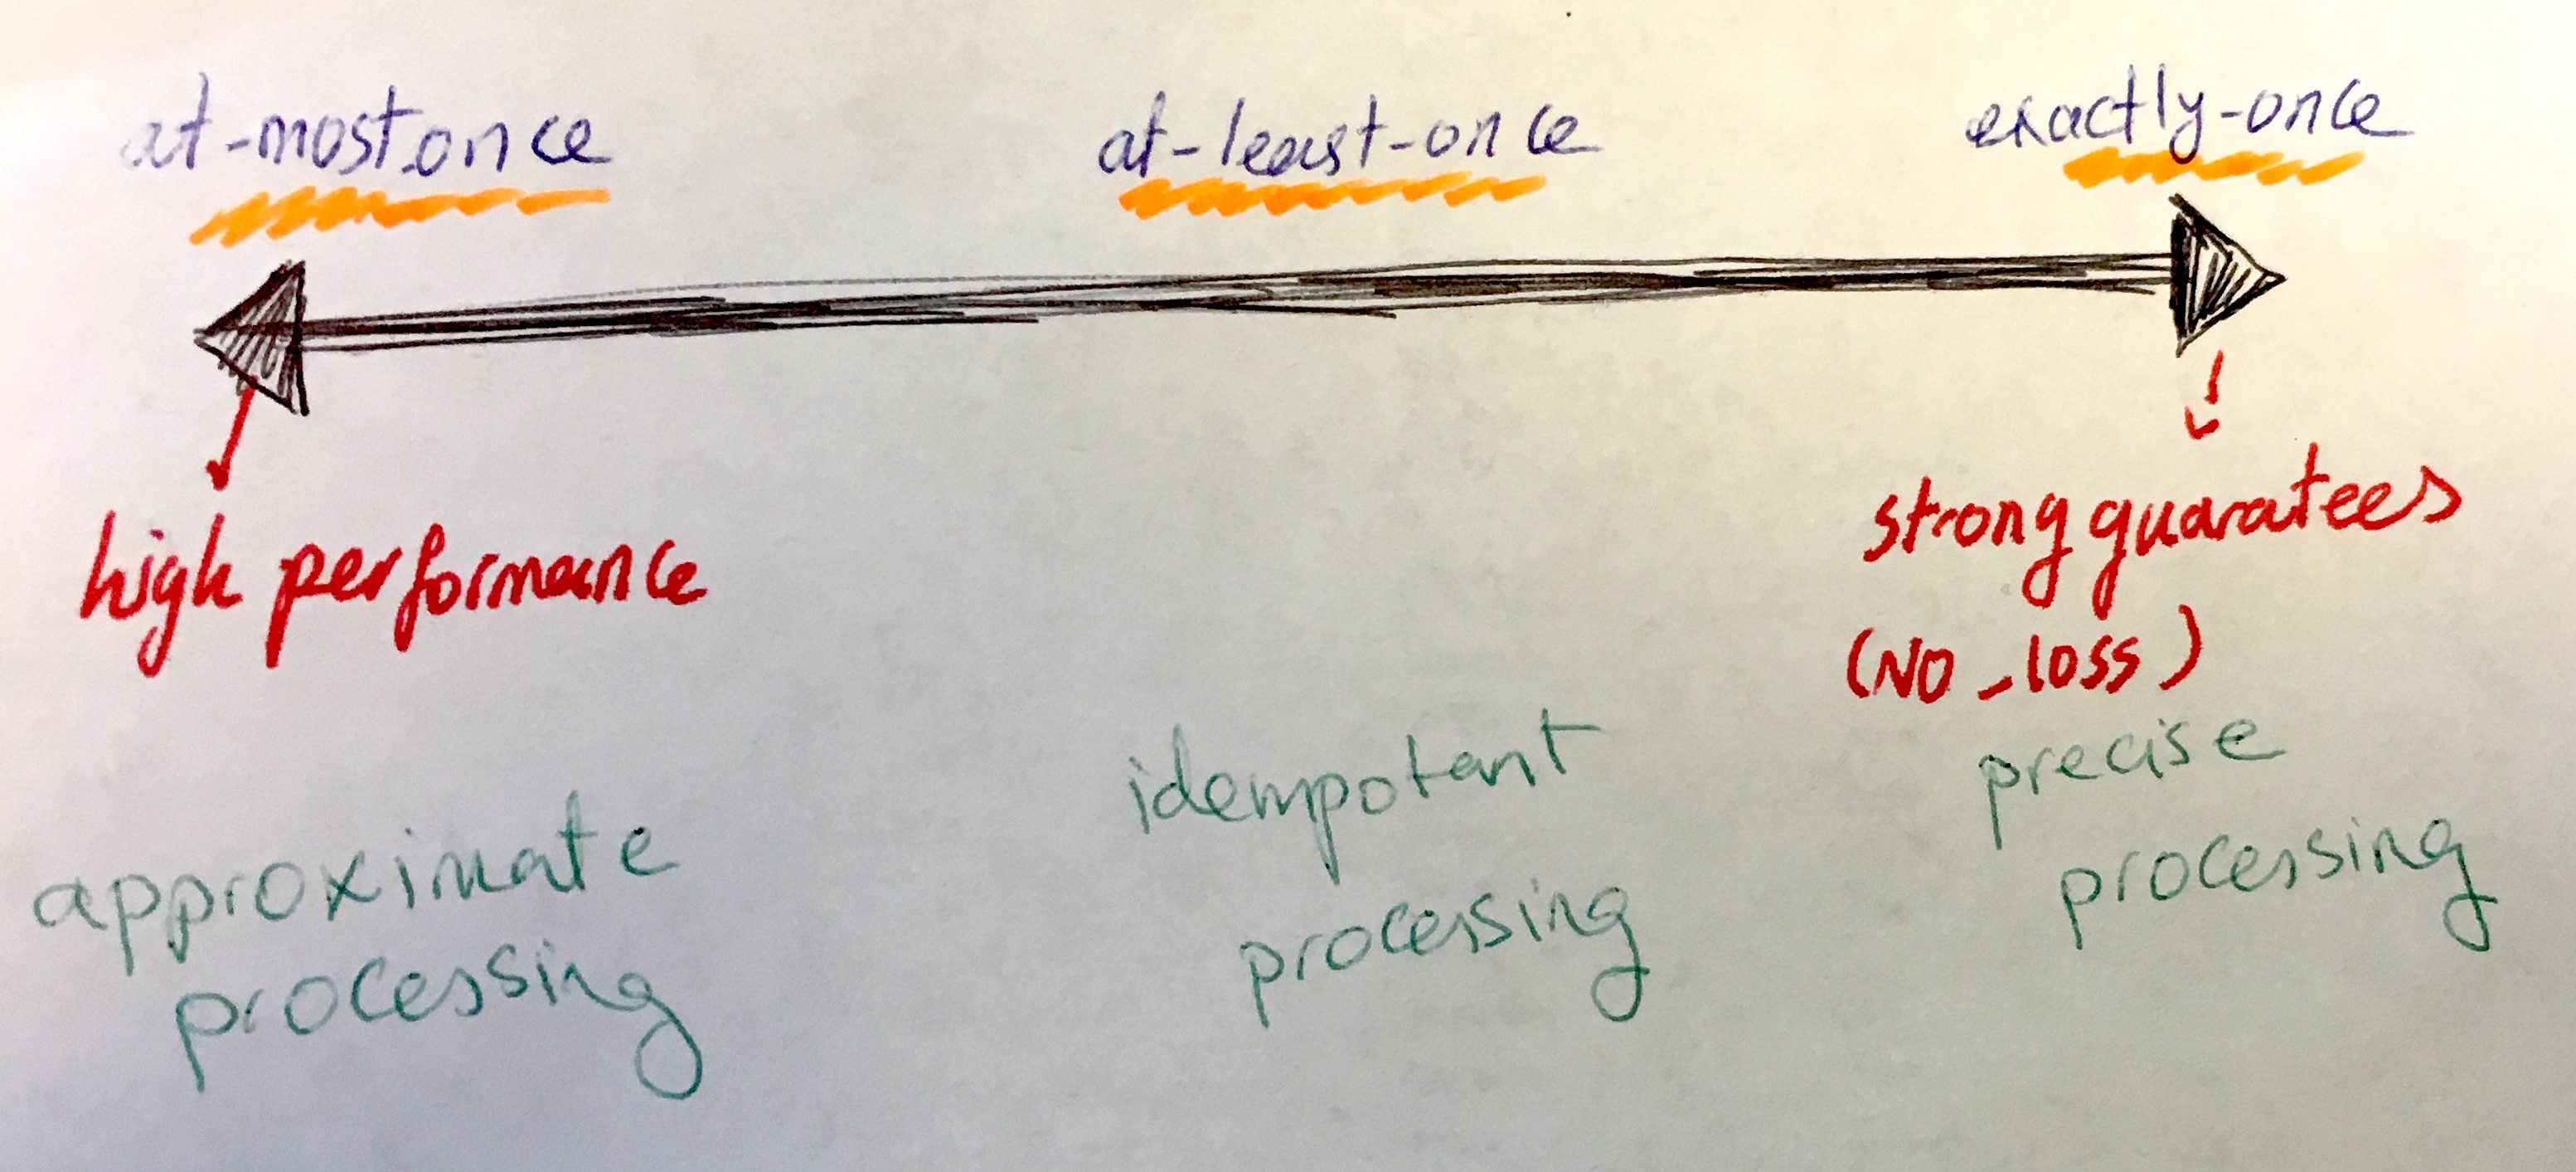
\includegraphics[width=0.45\linewidth]{guarantees.jpg}
		\caption{Spectrum of various guarantees and the trade-off among them.}
		\label{fig:guarantees}
	\end{figure}
	
	
	\noindent \textbf{Use-case:} at-most-once is good for approximate computing. Examples are: \Fix{...}. at-least-once is good for idempotent computations. in most cases ordering is preserved, and a series of messages are replayed. \Fix{is that true?}. Examples are: \Fix{...}.  exactly-once is good for cases that precise computation is needed. Examples are: \Fix{...}\\
	

\noindent \textbf{Solutions \& trade-offs:} at-most once, essentially means not adding any feature to the system. at-least once mechanism are: 1. using an (XOR based) acking. 2. using ordered messaging, with latest offset processed and replay when ever missing. 3. ?

exactly-once mechanism: 1. keeping track of all message ids processed, and check before reprocessing. 2. using total ordering, and detecting missing messages and re-requesting them 
\Fix{TODO: complete the selections} \\

\begin{table}[h]
	%\centering
	\tbl{Solutions to providing streaming gurantees and their trade-offs	\label{table:gurantee-summary}}{
		%		\begin{tabular}{|p{.1 \linewidth}|p|p|p|p|p|p|p|p|p|p|p|p|}%
		\tiny
		%	\begin{tabular}{|p{.09 \linewidth}|p{.05 \linewidth}|p{.05 \linewidth}|p{.05 \linewidth}|p{.05 \linewidth}|p{.05 \linewidth}|
		%	p{.05 \linewidth}|p{.05 \linewidth}|p{.05 \linewidth}|p{.05 \linewidth}|p{.05 \linewidth}|p{.05 \linewidth}|p{.05 \linewidth}|}%
		
		\begin{tabular}{|p{.1 \linewidth}|p{.15 \linewidth}|p{.3 \linewidth}|p{.3 \linewidth}|}%
			
			\hline
			\rowcolor[HTML]{E0E0E0} 
			Feature	&Solution	&Pros&Cons 
			\csvreader[head to column names]{tables/guarantee-summary.csv}{}% use head of csv as column names
			{\\\hline\textbf{\csvcoli} & \csvcolii & \csvcoliii &\csvcoliv }% specify your coloumns here
			\\ \hline
		\end{tabular}	
	}
\end{table}

 
\noindent \textbf{Future Direction:} current exactly once mechanism introduce too much overhead, especially in a system with high throughput. It is desirable to build a lower overhead mechanism. 






